\documentclass[11pt]{article}

\usepackage{style}

\title{Assignment 2}
\author{William Wang ww7964}
\date{February 20, 2020}

\begin{document}

\maketitle

\section{Approach}
In this lab we implemented an integer binary search tree and sequential/parallel hashing and comparison algorithms for our trees in Go. We primarily used channels and sync.WaitGroup as our synchronization primitives; additionally, we designed our own concurrent buffer based on sync.CondVar and sync.Mutex for distributing work items among worker goroutines.

\subsection{Data Structures}
Our BST implementation was fairly straightforward, consisting of Node objects containing a value, left pointer, and right pointer. The tree itself supported sequential insert, hash, and equals operations. These were implemented using a custom Stack to avoid recursive overhead.

To aid in grouping trees by their hashes, we designed the BucketMap, a list of maps from hashes to lists of tree IDs. This allowed us to parallelize the insertion of trees into groups without mutex protection, as we will see shortly.

\subsection{Hash and Group}
To compute a tree's hash, we performed an inorder traversal and accumulated a hash value as described in the problem statement. We did not attempt to parallelize this computation, but we were able to parallelize the creation of hash groups, i.e. the assignment of each tree to a set containing exactly those trees with an equivalent hash.

We represented hash groups using a map from hashes to lists of tree IDs having that hash. We explored three approaches for building this map:

\begin{enumerate}
    \item \textbf{Sequential:} Main thread calculates hashes for each tree and inserts into the map.
    \item \textbf{Mutex:} Main thread spawns some worker threads, each of which calculates and inserts items into the map. In this case, the map is protected with a mutex.
    \item \textbf{Central managers:} Main thread spawns worker threads and central manager threads. Worker threads compute hashes and deliver them to manager threads via channels. Manager threads insert items into the map. To ensure thread safety, we use a BucketMap with exactly one bucket per manager thread, meaning each sub-map is only inserted into by one manager. We achieve reasonable load balancing by making each manager responsible for those trees with $\text{hash} \equiv \text{manager-number} \pmod{\text{managers}}$.
\end{enumerate}

\subsection{Compare Trees}
After calculating our hash groups, we iterated through the trees within each group to rule out any possible hash collisions in our final groupings. Our sequential implementation was simply an inorder traversal of every pair of candidate trees, again using Stacks to store the traversal progress.

To parallelize tree comparisons, we started by spawning some worker threads and pointing them at a concurrent buffer, into which the main thread would insert work items in the form of tree ID pairs. Whenever a worker thread received a tree pair, it would spawn two more threads to walk the trees in lockstep. These threads communicated across a channel of pointers to check the trees' values against each other, with each thread doing exactly one send and receive.\footnote{To prevent deadlock, one thread was designated the ``first sender" and the other the ``first receiver".} When the end of the tree was reached by a thread, a nil pointer was sent instead. Thus, if either thread received an inconsistent value at any step of the traversal, it was guaranteed that both threads would exit. Only if both threads sent and received nil at the last step would the trees be marked equivalent.

\subsection{Concurrent Buffer}
Our concurrent buffer, BoundedBuffer, behaved exactly like a buffered Go channel. A call to \texttt{push(elem)} would attempt to insert an element and block if full, while a call to \texttt{pop()} would attempt to remove an element and block if empty. This was accomplished using a circular array protected by two condition variables, which represented whether the buffer was empty or full. \texttt{push} would wait on the full one and signal the empty one, and vice versa with \texttt{pop}.

\section{Analysis}
We tested and profiled our program on a 4-core, 8-thread machine by executing our code 20 times on each of \texttt{simple.txt}, \texttt{coarse.txt}, \texttt{fine.txt} for combinations of hash-workers, data-workers, comp-workers in the range $\{1, 2, 4, 8, 16\}$. The below results are of the average running times within each set of 20 trials.

\subsection{Hash Computation (Figure 1)}
For the simple dataset, we observed no scaling at all; understandable given the tiny size of the input, causing parallel overheads to dominate. In fact, this happened for every type of computation measured. On the other hand, we achieved decent scaling for the coarse and fine datasets, leveling off around 8 threads - the number of hardware threads available. 

\begin{figure}[t]
    \centering
    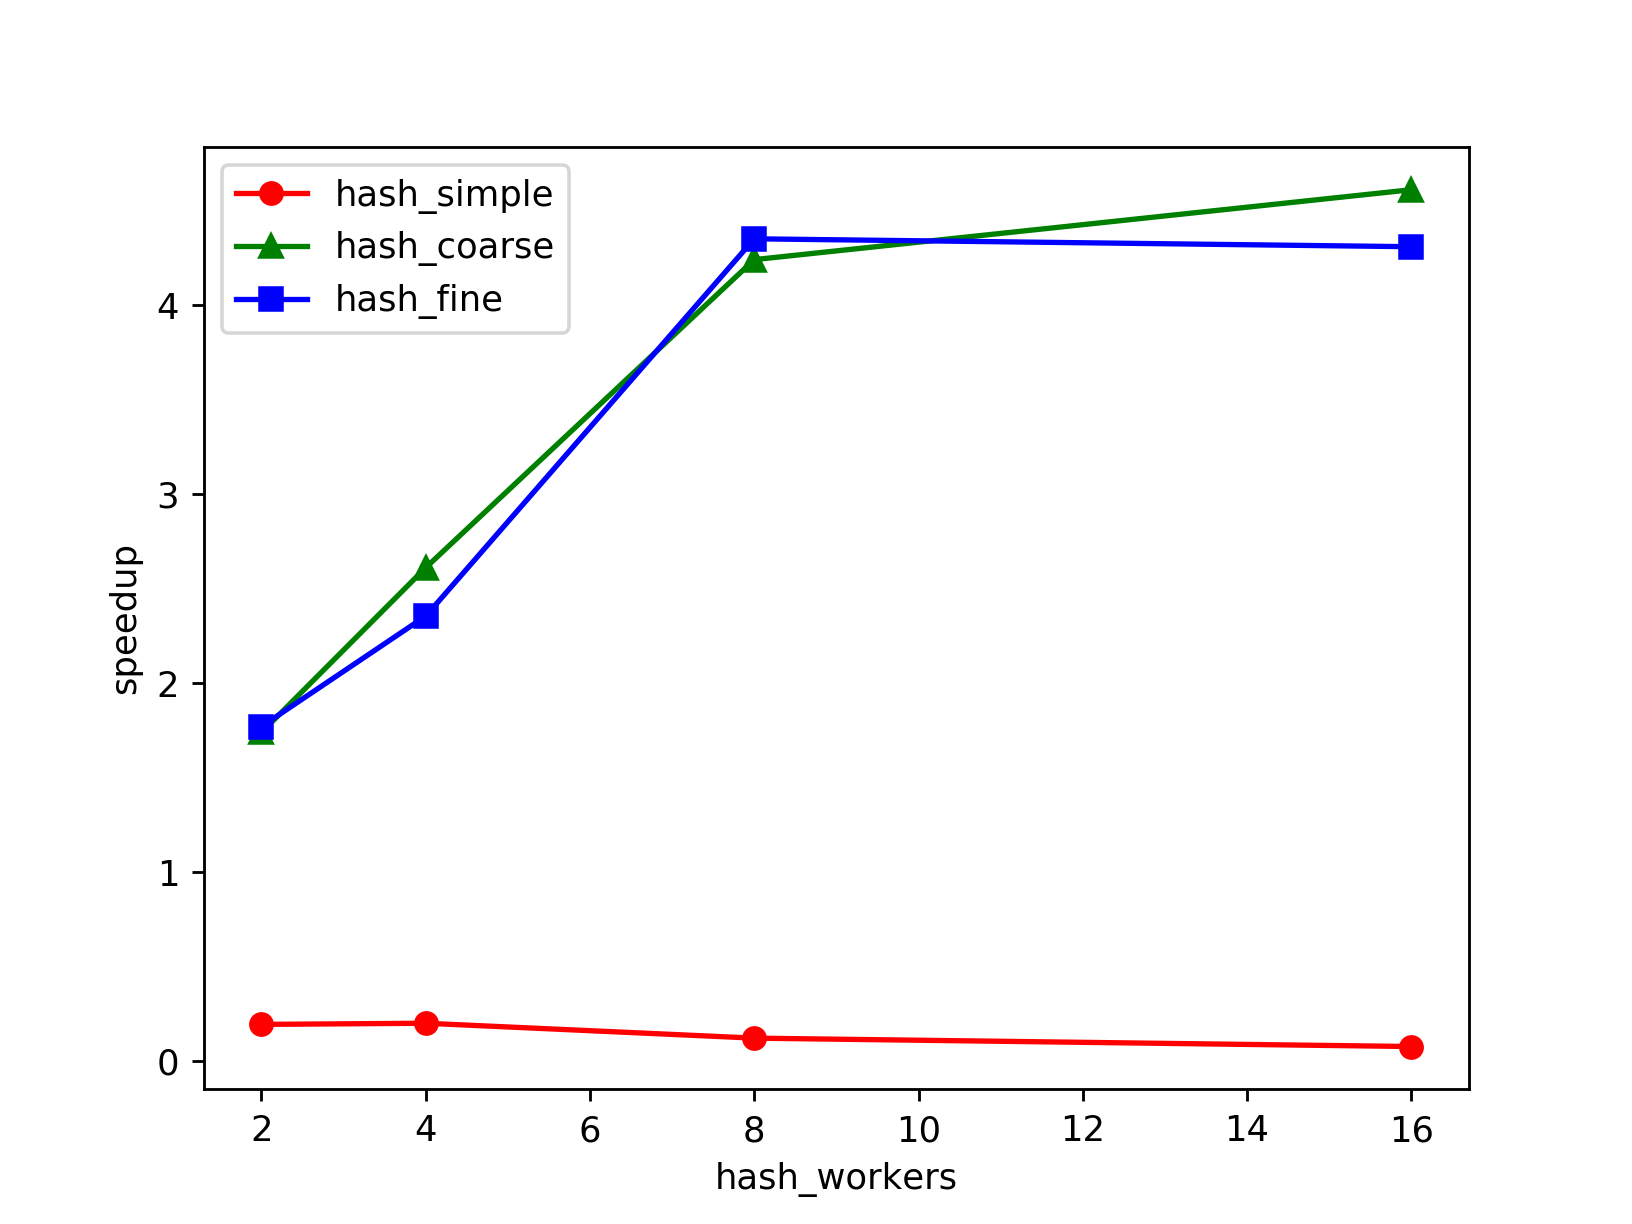
\includegraphics[width=5in]{media/hash.png}
    \caption{Hash computation speedup vs. threads}
\end{figure}

\subsection{Tree Comparison (Figure 2)}
In our tree comparison code, the results were flipped: the fine dataset achieved better scaling than the coarse dataset. We suspect that this was due to the limitations of a single concurrent work buffer under a large number of trees. Because each tree pair needed to go through the buffer, the rate at which work could be taken out of the buffer became the limiting factor. In the fine dataset, with a much larger number of tree pairs being pushed into the buffer, the net effect of each additional consumer thread/buffer slot was magnified. This allowed us to achieve high scalability; however, the total running time was still terrible - as expected - with the fine dataset.

\begin{figure}[t]
    \centering
    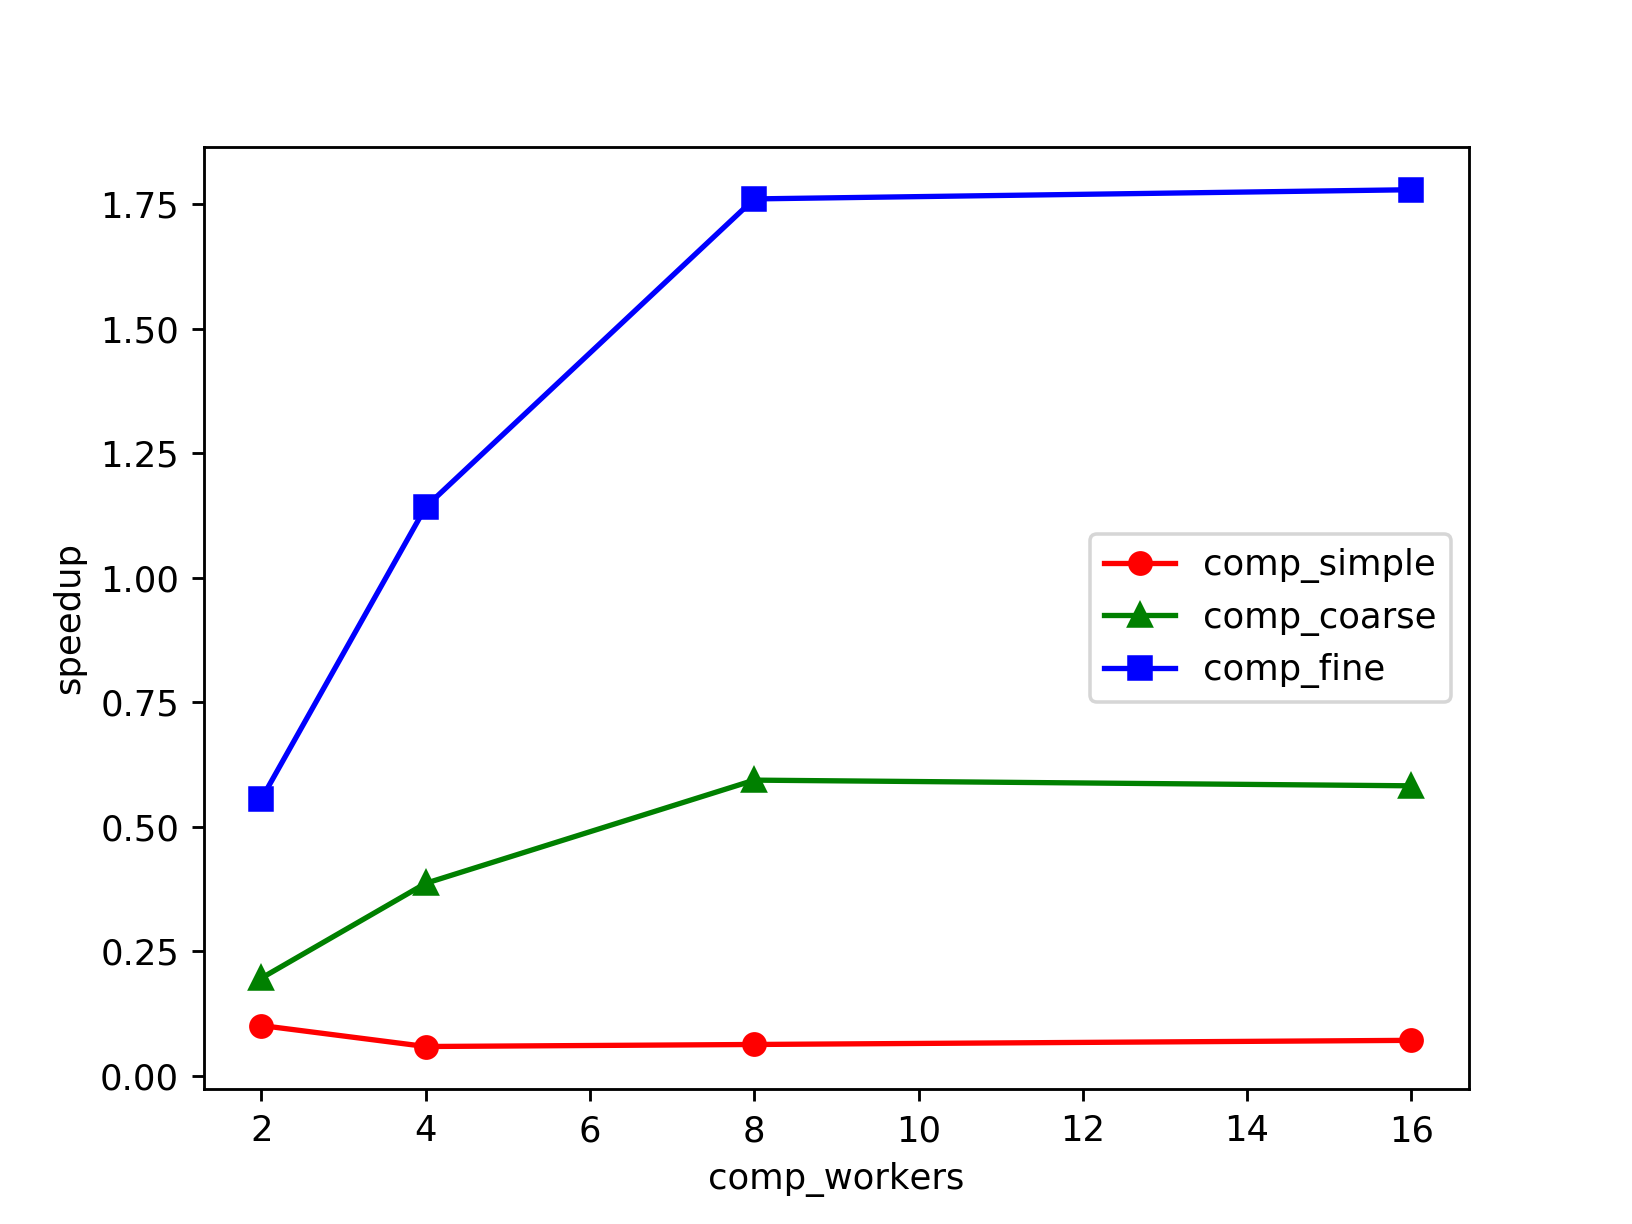
\includegraphics[width=5in]{media/comp.png}
    \caption{Tree comparison speedup vs. threads}
\end{figure}

\subsection{Hash Grouping (Figures 3-5)}
Hash grouping using a mutex around the map versus using a single central manager performed roughly the same, scalability-wise. The coarse dataset produced decent scaling up to 8 threads, likely because the work was dominated by the actual computation of hashes rather than ``logistical" issues, like inserting items into the map. The opposite was true of the fine dataset, where contention for the map across many inserting threads was the bottleneck. This situation differed from tree comparison in that increasing the number of hash workers did not also increase the effective bandwidth of the data stream going into the map, unlike our concurrent buffer which was sized for exactly the number of comparison workers. Hence, poor hash group scaling was observed for a large number of trees.

By the same argument, we can see why the fine dataset scales best when the number of hash workers is fixed and the number of central managers increases. We are effectively widening the bottleneck into the map when we increase the number of managers. Accordingly, the coarse dataset is not affected at all, as it remains bound by the actual computation of hashes.

\begin{figure}[t]
    \centering
    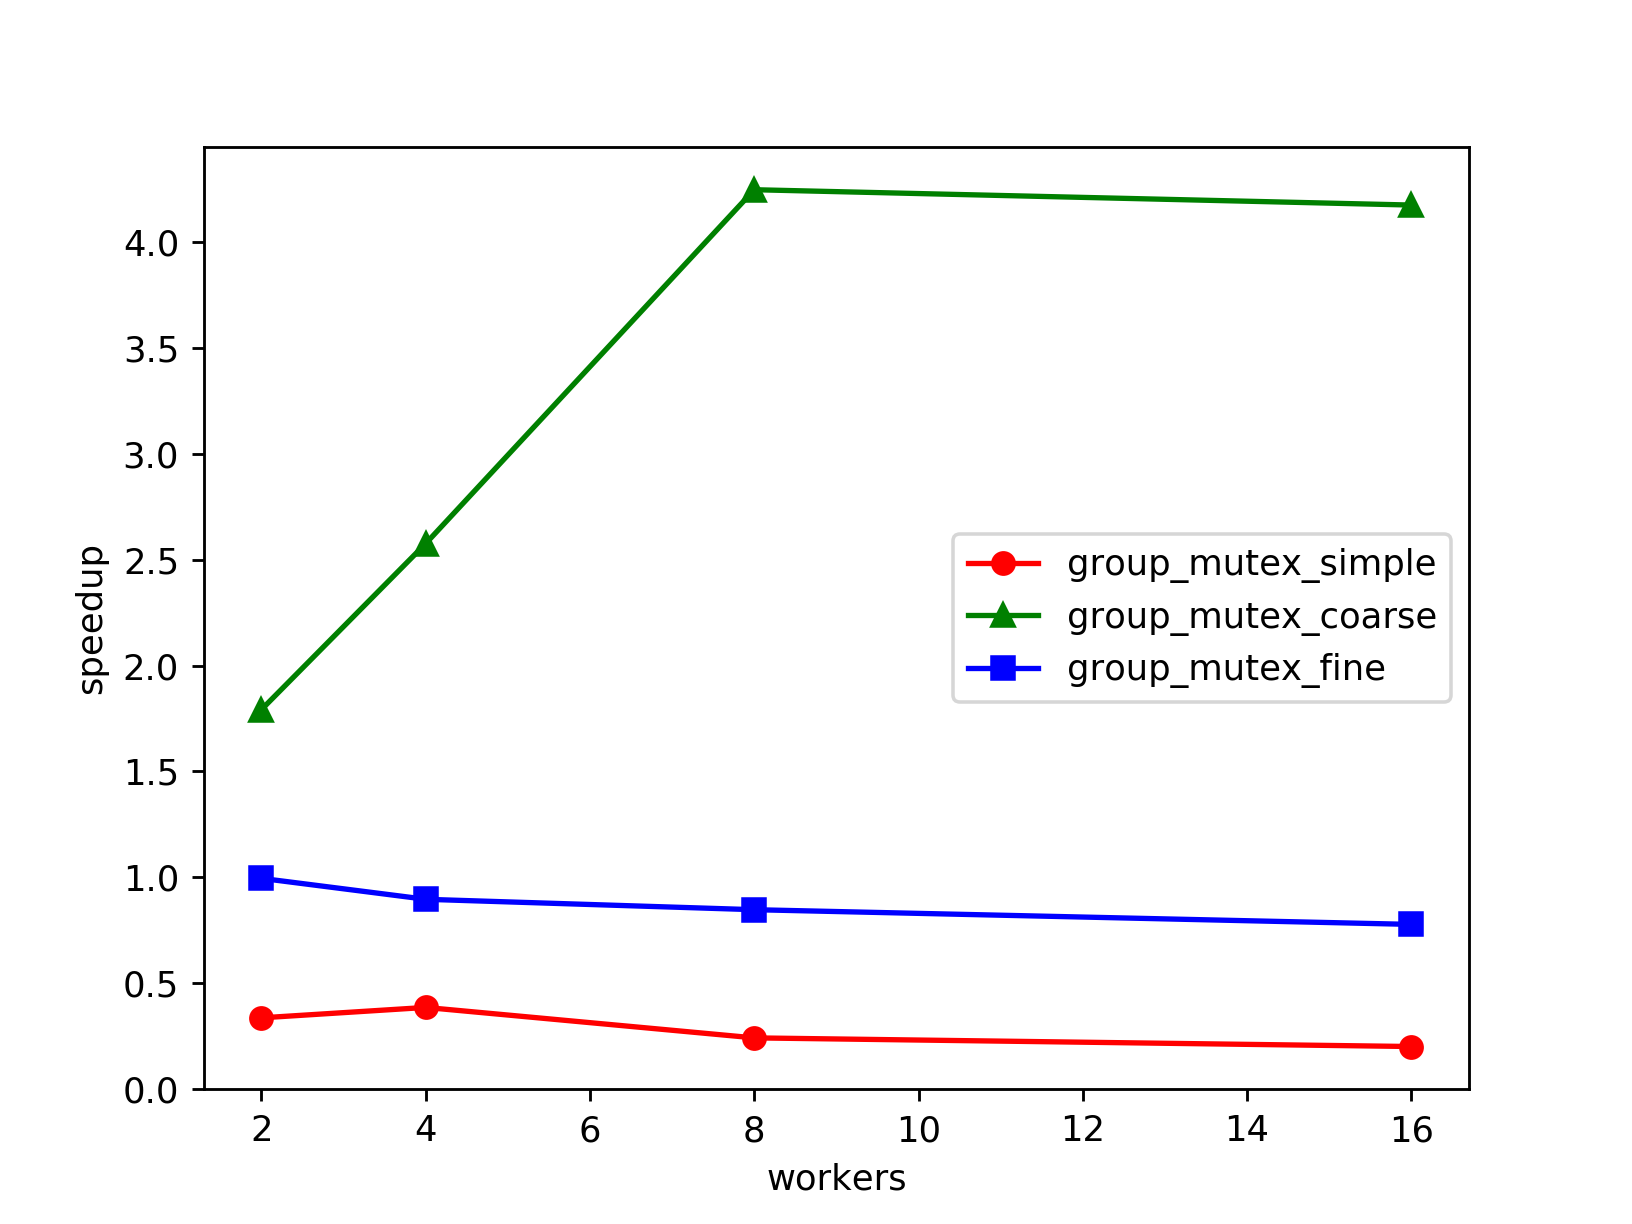
\includegraphics[width=5in]{media/group_mutex.png}
    \caption{Hash grouping (using mutex) speedup vs. threads}
\end{figure}

\begin{figure}[t]
    \centering
    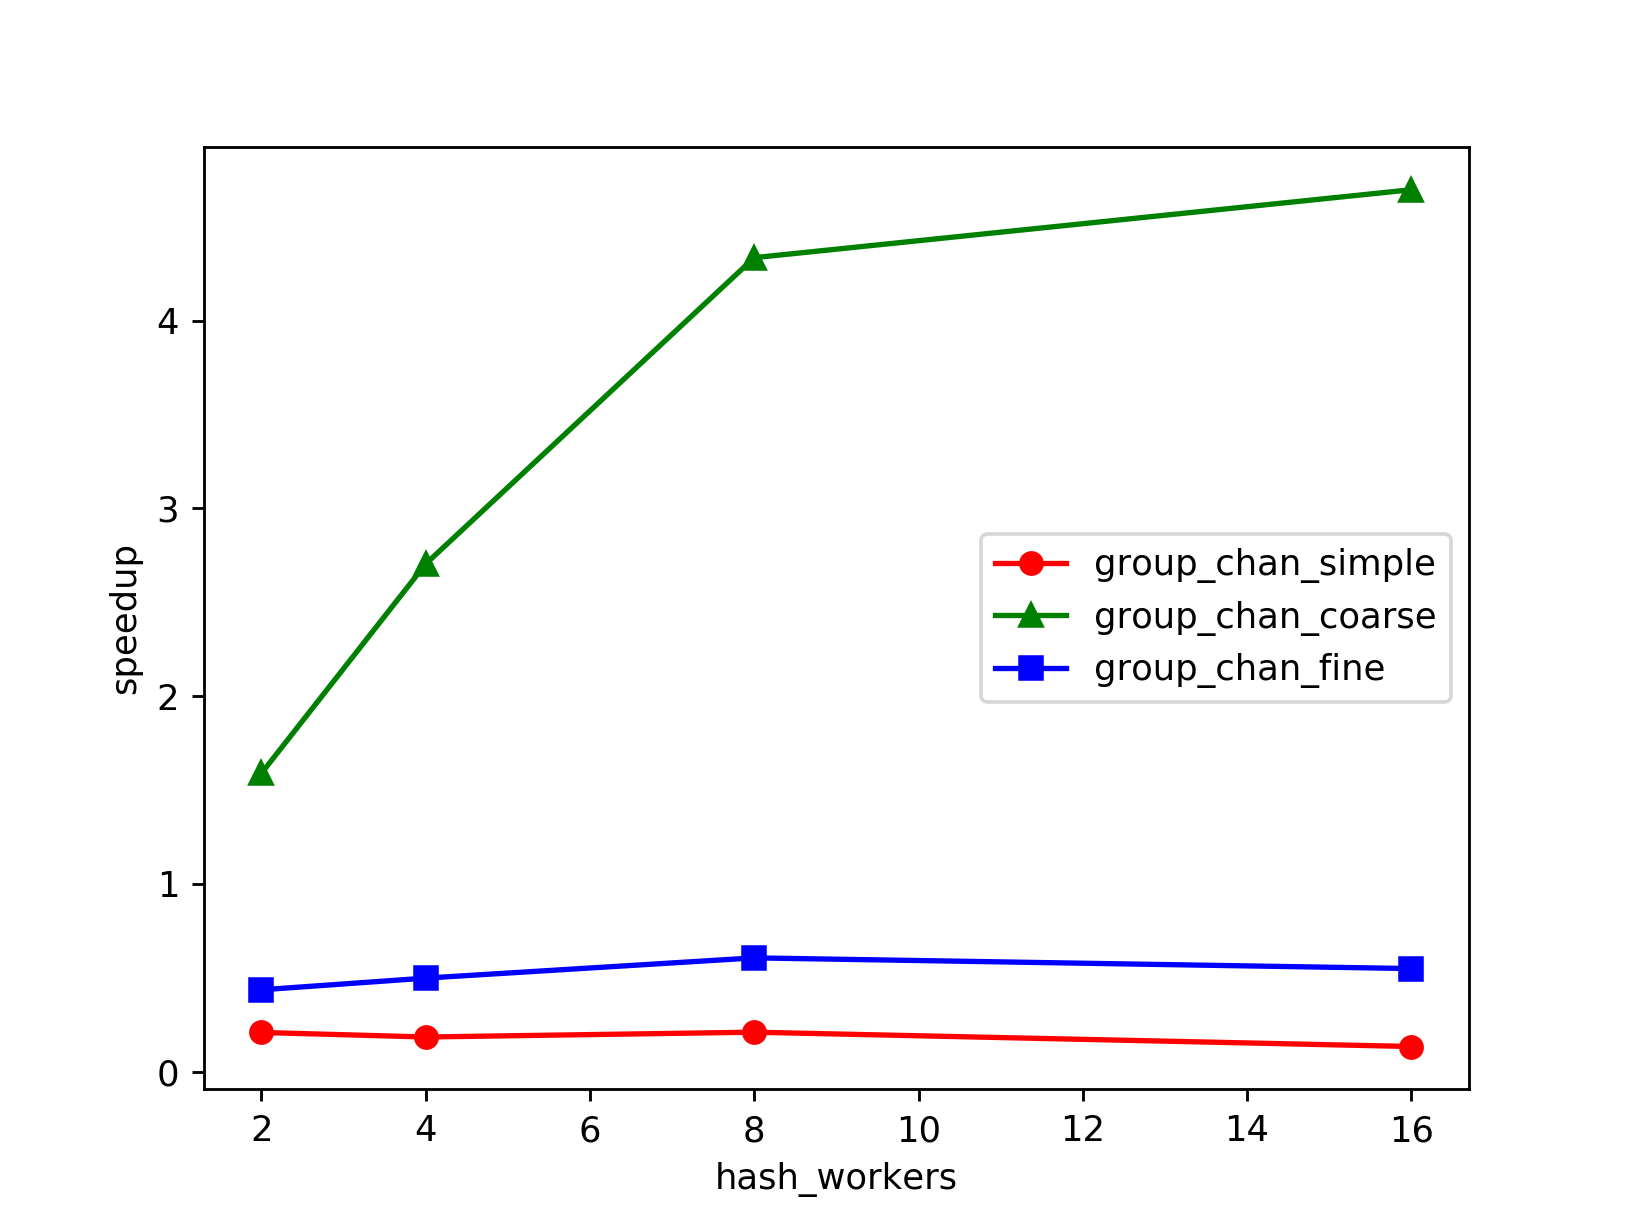
\includegraphics[width=5in]{media/group_chan.png}
    \caption{Hash grouping (using single manager) speedup vs. threads}
\end{figure}

\begin{figure}[t]
    \centering
    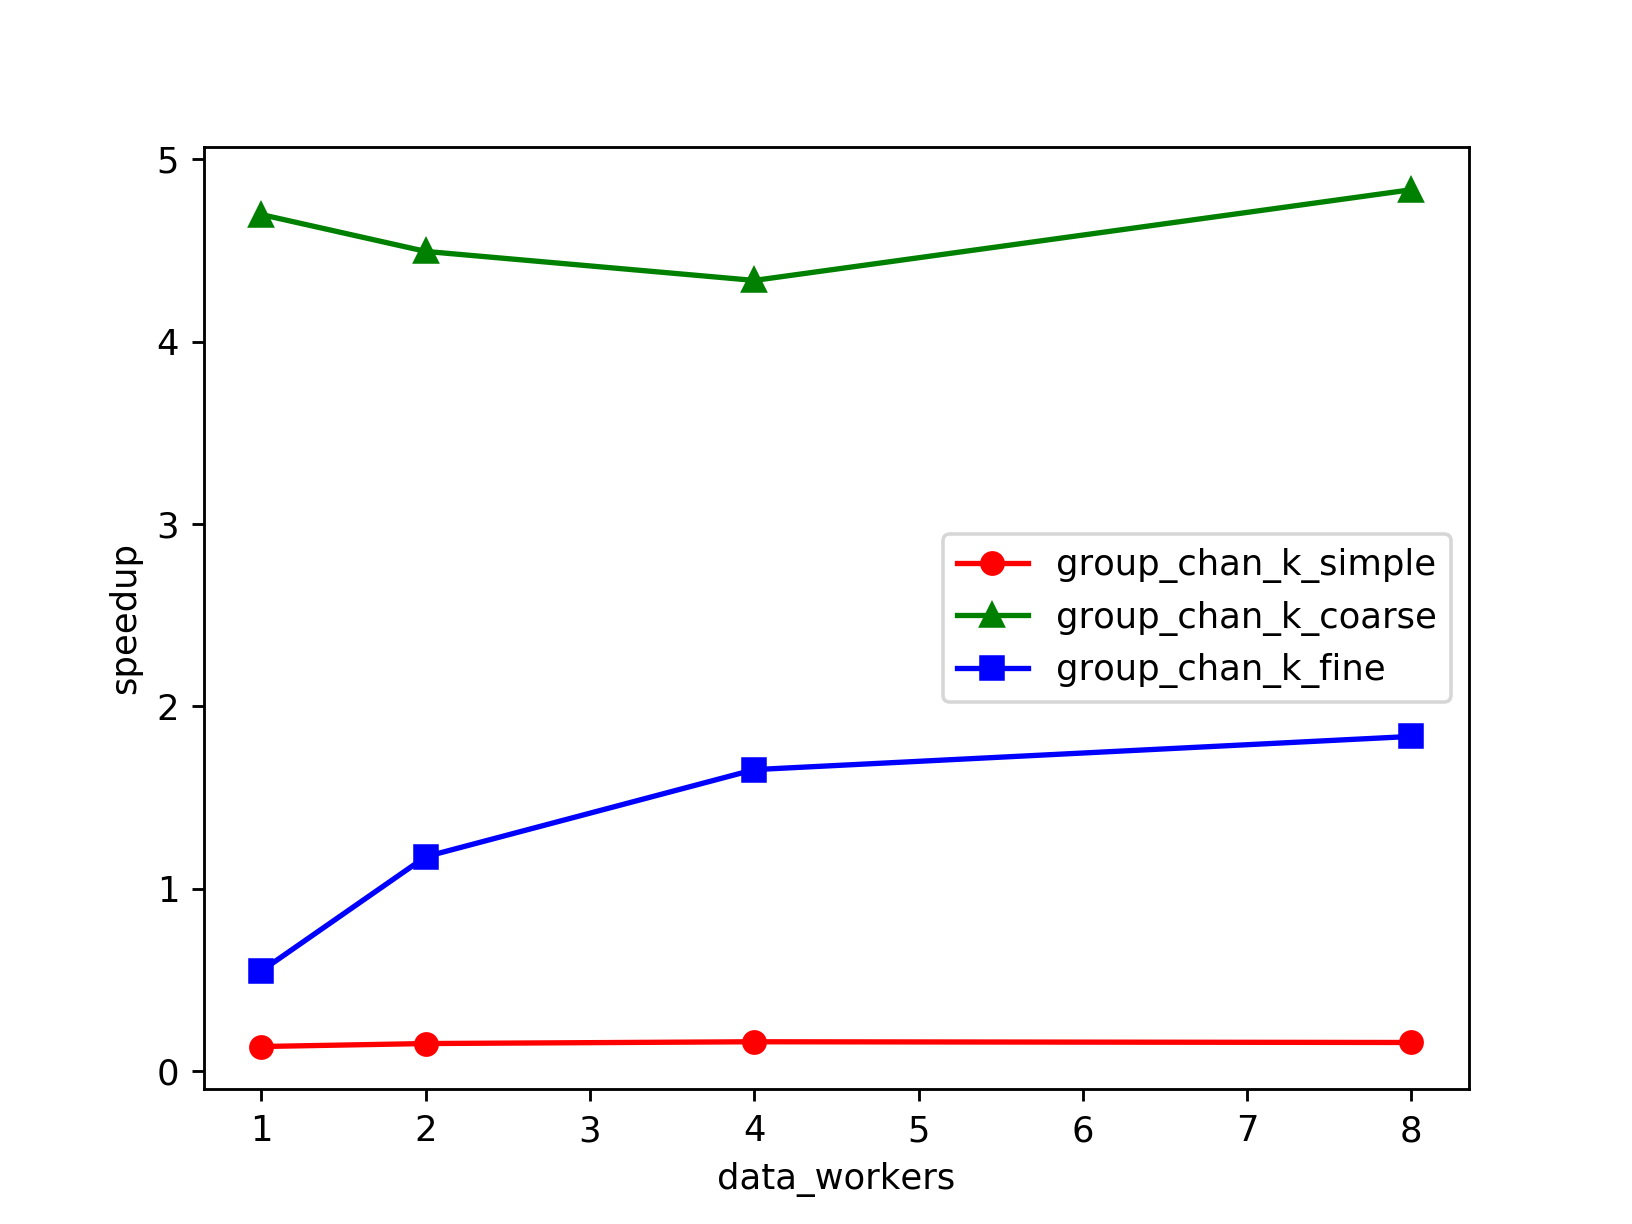
\includegraphics[width=5in]{media/group_chan_k.png}
    \caption{Hash grouping (using variable managers with 16 hash workers) speedup vs. threads}
\end{figure}

\section{Insights}
One of our biggest challenges was telling worker threads to stop and synchronizing with them properly. Each worker effectively used channel receives to synchronize, so after the last value was received, it would block forever. We could send a poison value across the channel to tell the worker to stop, but with all integer data being valid, we couldn't reliably choose one. The approach we decided on was to add a level of indirection and send pointers across our channels, with a nil pointer being the poison value. Even so, we had to fix a number of race conditions,  However, Go is so good at load balancing goroutines that over all our test runs, we never saw this race actually have an effect on our program output. 

Overall, we were extremely impressed with the lightweight-ness of goroutines and channels. In our profiling, we observed that channels in excess of hardware threads (8) didn't hurt performance at all. Moreover, the scaling before that point was essentially a straight line in most cases, implying a tiny overhead associated with creating and synchronizing goroutines. 

\end{document}
